\section*{Soft Tasks}
\subsection*{Correlation Analysis}

\todo{}

\begin{figure}
\centering
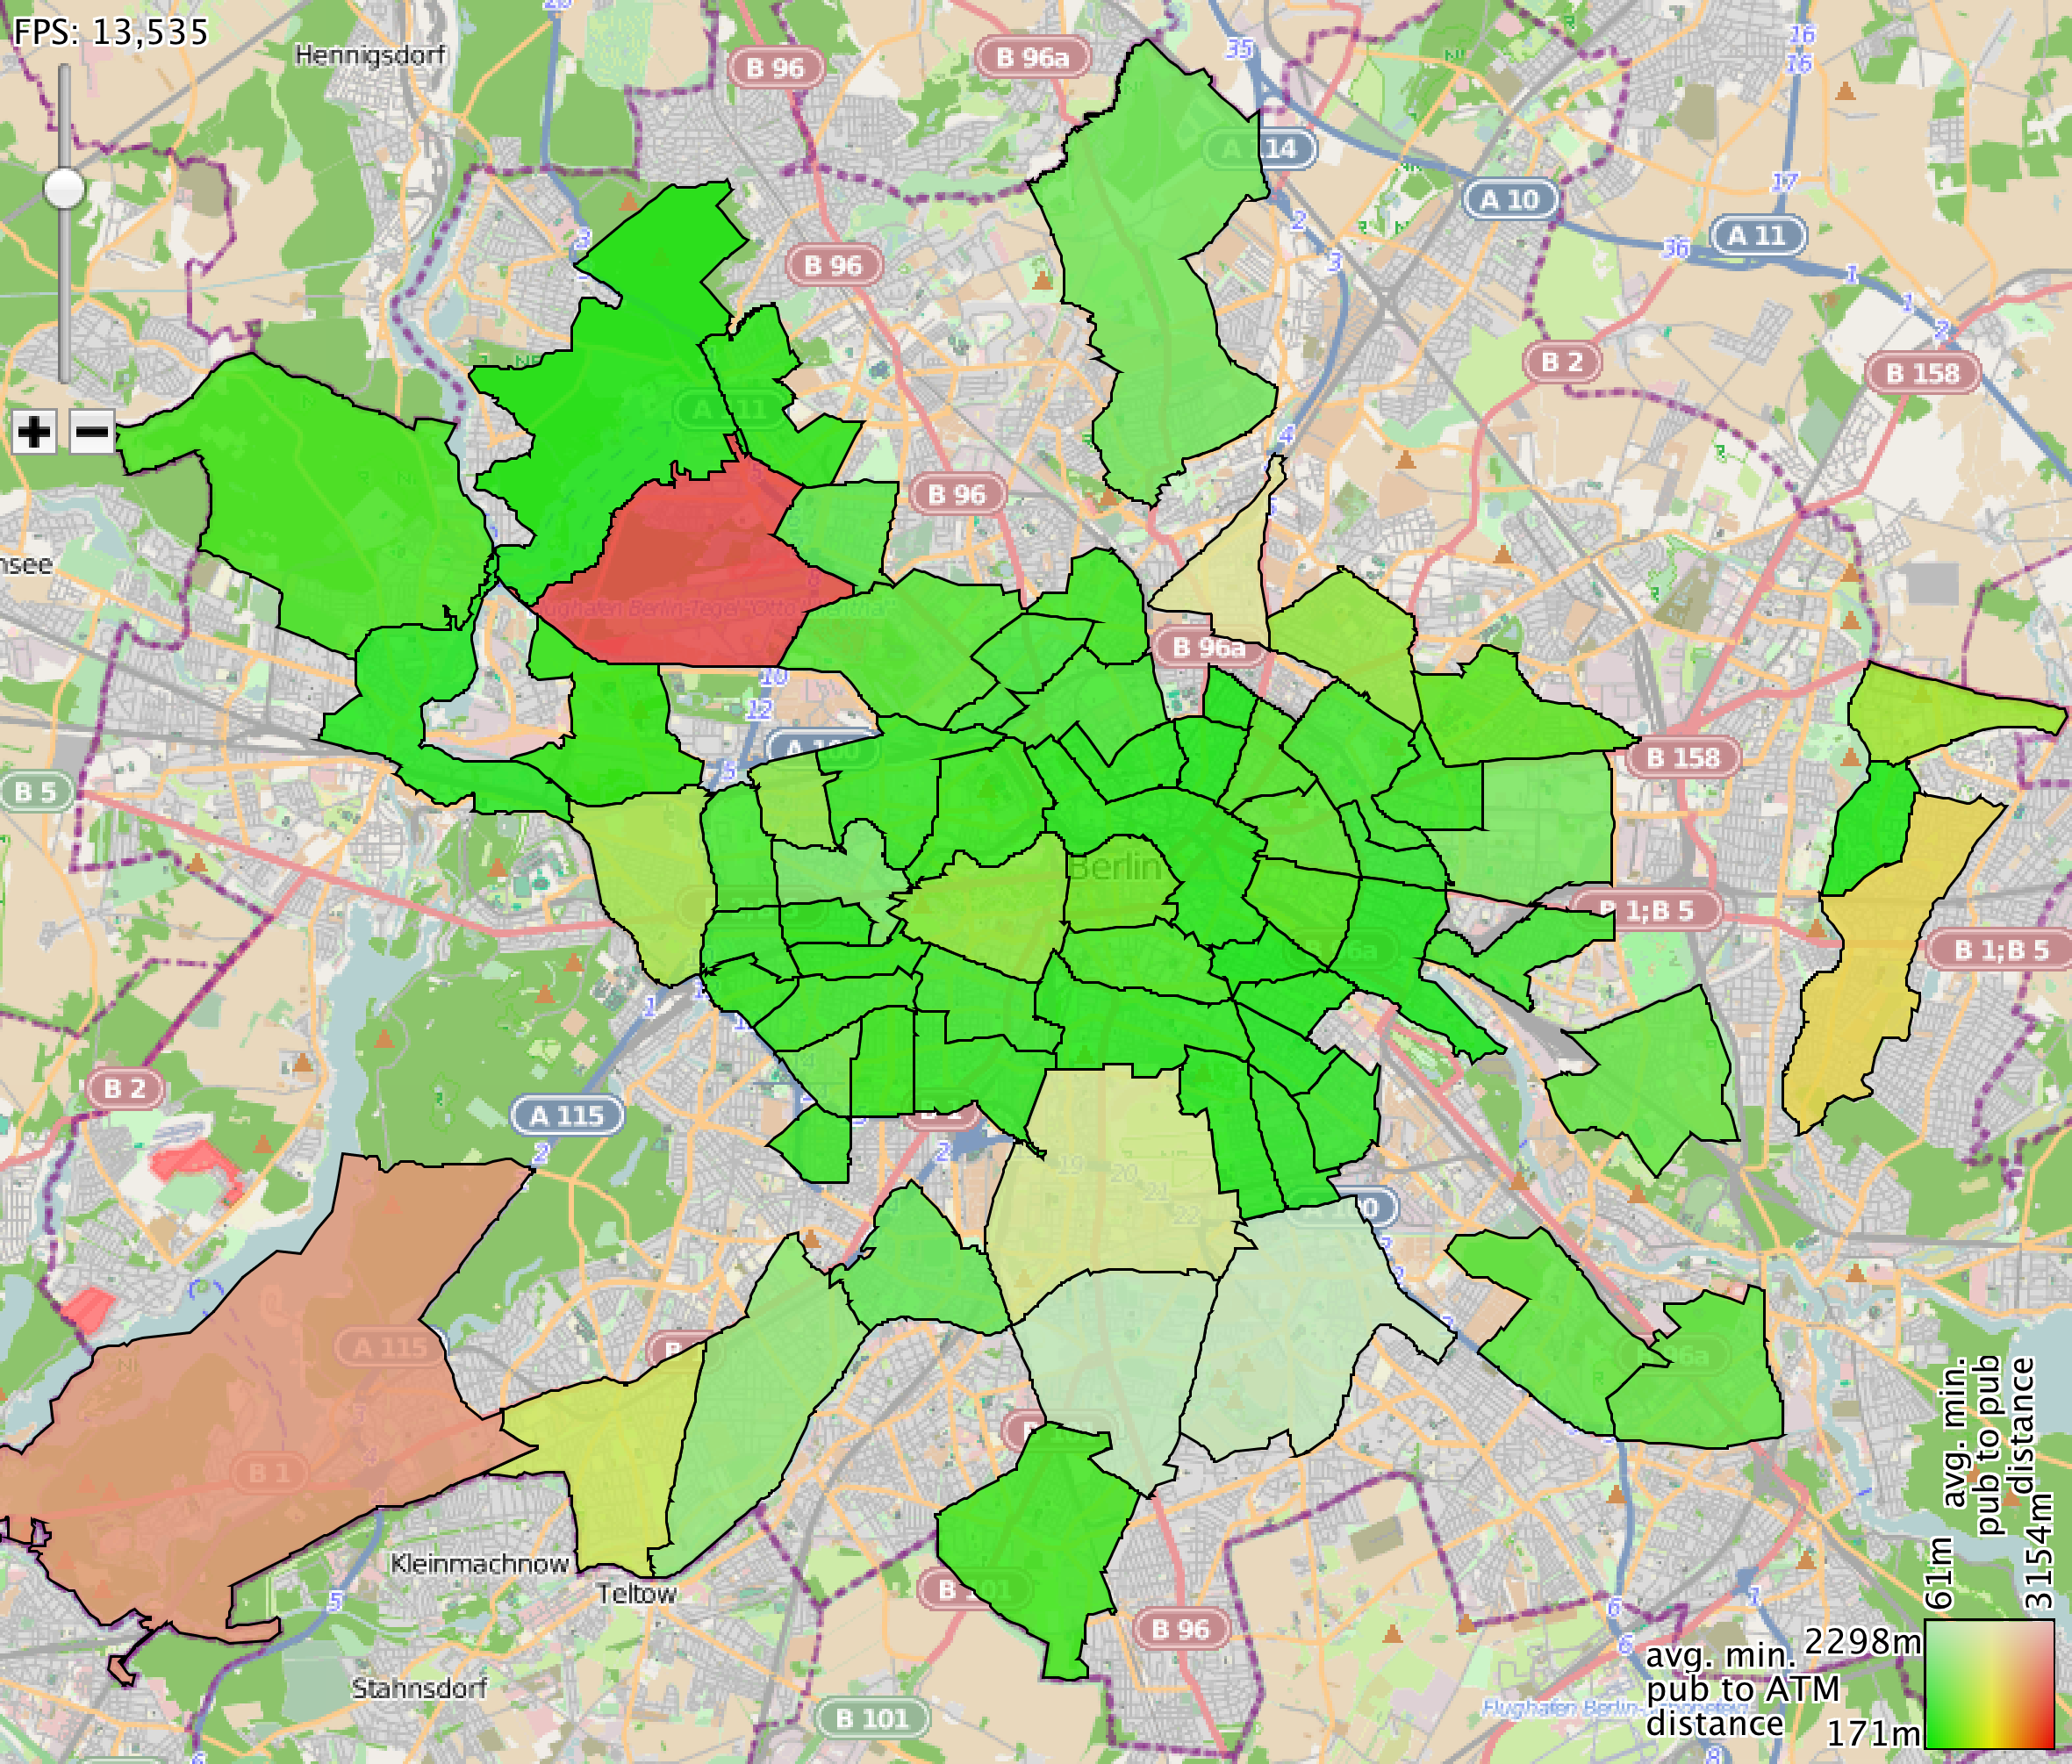
\includegraphics[width=0.9\linewidth]{imgs/crawl}
\caption{\todo{}}
\label{fig:crawl}
\end{figure}

\subsection*{Open Wi-Fi}

As additional dataset we use data of open and free Wi-Fi hotspots in
the area of Berlin.
The data is displayed as heatmap.

The dataset originally consisted only of plain-text street addresses
of buildings with open Wi-Fi hotspots. We converted the
address data into building polygons via the Google Maps
API and the buildings from the OSM dataset.

The heatmap is computed in a mesh of
arbitrary size. Each cell is computed by adding
the nearest distances of all buildings with a Wi-Fi
hotspot together.
Since this is computationally expensive ($\mathcal{O}(whn)$ where $w$ and $h$
are the width and height of the mesh respectively and $n$ is the total number of lines
defining all buildings with Wi-Fi)
we start with a loose mesh and refine it up to one pixel per cell while the
user is inactive.

Looking at the heatmap reveals some areas with higher density of open hotspots.
Namely the center of the city (Mitte), around the Sony Center, in Prenzlauer Berg, and
in the area around Simon-Dach-Str. in Friedrichshain.
Those areas are known for being touristic and Mitte with Sony Center are additionally
areas with many businessmen.
As hotspots are likely to be in a restaurant, bar, or caf\'{e}
this seems to be due to the high demand for internet
of tourists (having no alternative) and businessmen (needing to
be online during lunch).

\begin{figure}
\centering
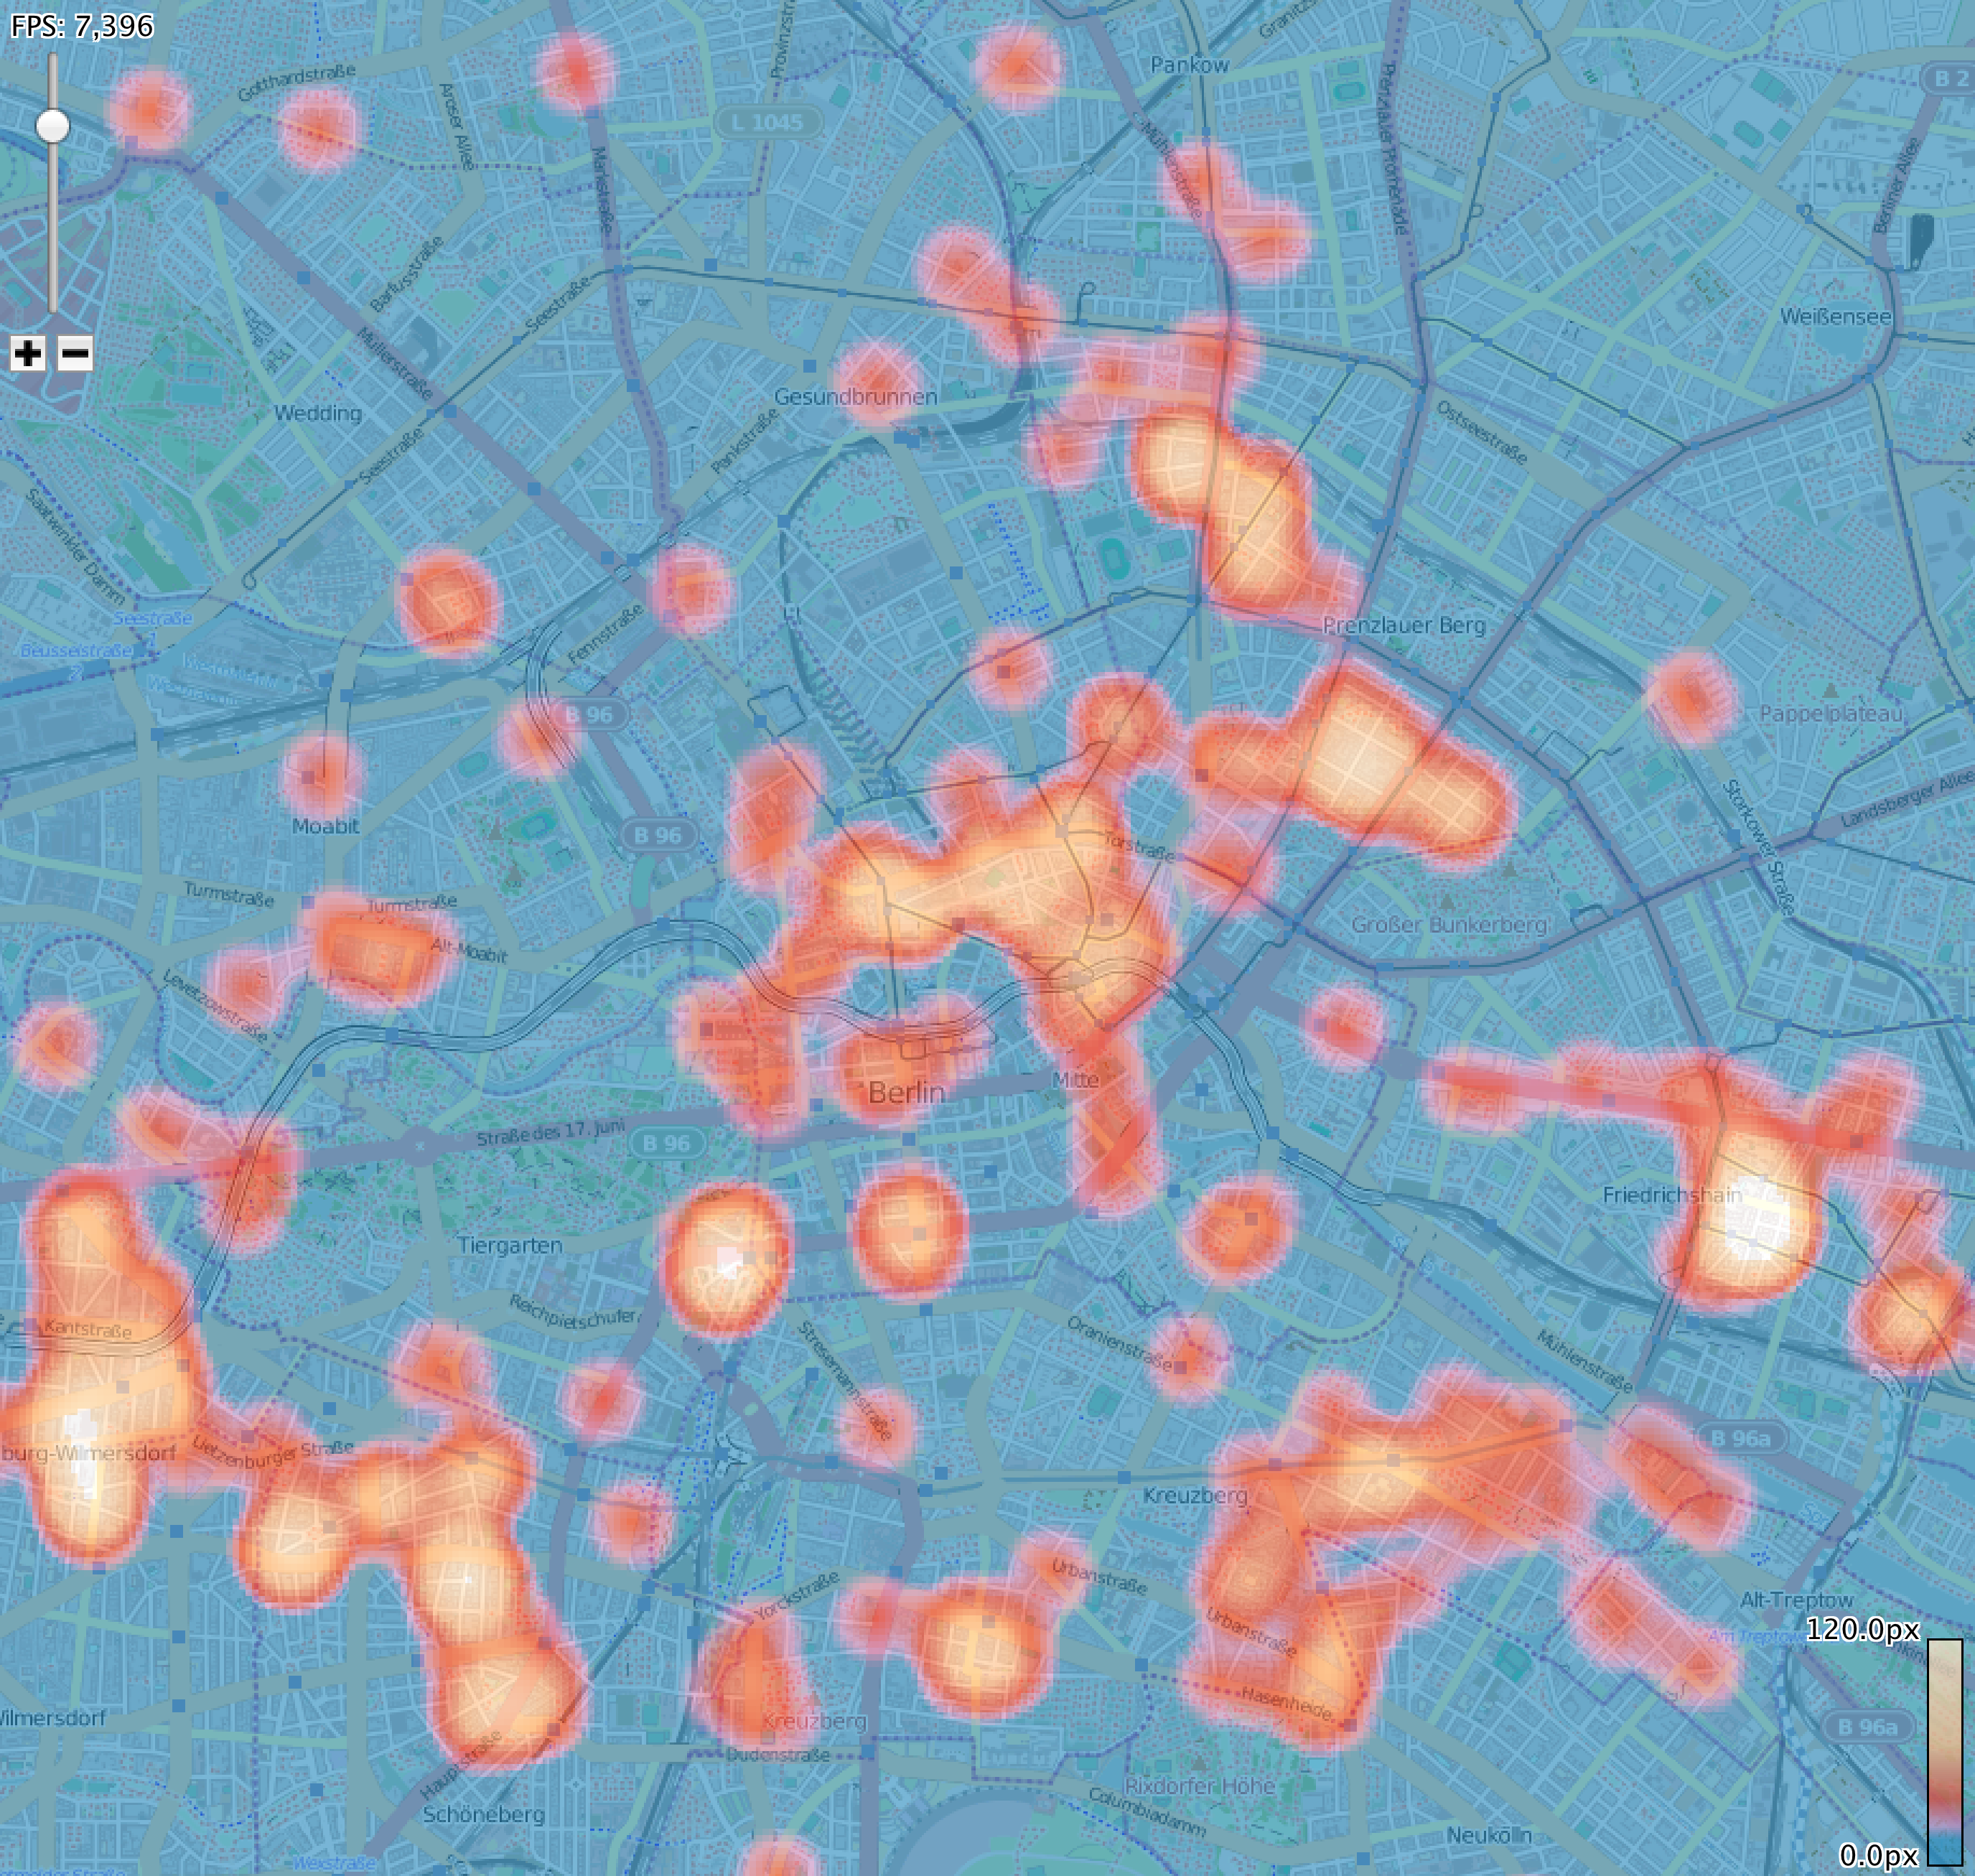
\includegraphics[width=0.9\linewidth]{imgs/heat}
\caption{The heatmap of open and free hotspots in Berlin.
The white spot to the right is the area around Simon-Dach-Str.}
\label{fig:heat}
\end{figure}
